\documentclass[conference]{IEEEtran}
\usepackage{amsmath,amssymb,booktabs,graphicx,url,cite}
\usepackage[T1]{fontenc}
\hyphenation{CSMA}

\begin{document}
\title{Reward Design Determines Whether Independent DQN Agents Learn Useful Contention Windows in CSMA/CA}

\author{\IEEEauthorblockN{Hesam Amiri}
\IEEEauthorblockA{Department of Electrical, Electronic, and Information Engineering\\
University of Bologna, Bologna, Italy\\
hesam.amiri@studio.unibo.it}}
\maketitle

\begin{abstract}
Binary exponential backoff (BEB) in CSMA/CA ignores network density, which makes learning the contention window (CW) an attractive application of deep reinforcement learning, yet reported results are mixed. We study this question in a slotted CSMA/CA simulator that we validate against Bianchi's analytical model. Each node runs a Deep Q-Network (DQN) that selects its CW from local observations only. We find that the outcome is dominated by the reward design rather than by the learning algorithm. With a local reward that penalises waiting time, independent agents choose CWs that are too small and collapse: at $N{=}20$ saturated nodes the throughput is @@b01i20@@ versus @@beb20@@ for BEB. A team reward, the system utilisation observed only during training, lets independent agents improve on BEB at every tested density (by up to @@dmax@@) and match the best static CW, but at a large fairness cost (Jain index @@jti20@@ at $N{=}20$). Parameter sharing keeps fairness (@@jts20@@) and still improves on BEB at most densities, but is less stable at high density. A single learner among BEB nodes exposes the mechanism: it takes @@sh20_01@@ times its fair share of successes under the local reward and @@sh20_t@@ times under the team reward. Results are averaged over 10 seeds with paired significance tests.
\end{abstract}

\begin{IEEEkeywords}
medium access control, CSMA/CA, contention window, deep reinforcement learning, reward design, multi-agent learning
\end{IEEEkeywords}

\section{Introduction}
In IEEE 802.11 CSMA/CA, a node doubles its contention window (CW) after every collision and resets it to $\mathrm{CW}_{\min}$ after every success. The rule is simple and robust, but it does not depend on the number of contending nodes, whereas the throughput-optimal transmission probability does~\cite{bianchi2000}. This gap motivates learning-based MAC protocols in which each node adapts its CW from local observations~\cite{amuru2015,wydmanski2021,yu2019}.

Reported outcomes are nevertheless mixed. Learning agents share a channel and therefore interact, so one may expect the difficulties of independent multi-agent learning, in particular non-stationarity~\cite{hernandez2017}, to explain failures. In this paper we test that expectation directly and find that, in our setting, a more basic factor dominates: \emph{what the agents are rewarded for}. Our contributions are:
\begin{itemize}
\item A validated, open slotted CSMA/CA simulator with counter-based backoff and freezing, together with strong non-learning references: BEB, the best static CW per network size, and an analytic oracle (Section~\ref{sec:model}).
\item A systematic comparison of independent and parameter-shared DQN agents under three reward designs, with 10 seeds, confidence intervals, paired tests, and fairness reported alongside throughput (Section~\ref{sec:results}).
\item A diagnostic experiment in which a single learner competes against BEB nodes, showing that local rewards produce greedy behaviour and team rewards produce altruistic behaviour (Section~\ref{sec:results}-E).
\end{itemize}

\section{Related Work}
Bianchi's Markov-chain model of the 802.11 DCF~\cite{bianchi2000} is the standard analysis of saturation throughput and underlies our baselines. Amuru et al.\ formulate the optimisation of the 802.11 backoff mechanism as a Markov decision process and propose a post-decision-state learning algorithm that exploits known protocol dynamics, reporting gains over BEB and over standard Q-learning~\cite{amuru2015}. Wydma\'nski and Szott apply deep reinforcement learning to contention-window optimisation in IEEE 802.11ax~\cite{wydmanski2021}. Yu et al.\ use a DQN to design a MAC protocol that coexists with TDMA and ALOHA networks, with a generalised $\alpha$-fairness objective~\cite{yu2019}. Our study differs in its focus: we hold the learner fixed (a small DQN~\cite{mnih2015}) and vary the reward and the degree of parameter sharing, using a simulator whose baselines we validate analytically.

In multi-agent reinforcement learning, treating other learners as part of the environment makes the problem non-stationary~\cite{hernandez2017}. Tampuu et al.\ showed that independent DQN agents behave competitively or cooperatively depending on the reward scheme~\cite{tampuu2017}, which is consistent with our findings. Centralised training with decentralised execution, e.g.\ MADDPG~\cite{lowe2017} and QMIX~\cite{rashid2018}, uses information available only during training; our team reward is a minimal instance of this idea. We do not evaluate those algorithms here.

\section{System Model and Baselines}\label{sec:model}
\subsection{Simulator}
$N$ nodes share one collision domain with perfect carrier sensing. Time advances in events: an idle slot lasts one slot, and a busy period (success or collision) lasts $T{=}20$ slots, as in Bianchi's $T_s{=}T_c$ setting. Each contending node draws a backoff counter uniformly from $\{0,\dots,\mathrm{CW}-1\}$; counters decrease only in idle slots and are frozen during busy periods; a node transmits when its counter reaches zero. One transmitter succeeds, two or more collide. Nodes are saturated (always backlogged). A new CW is chosen each time a node starts a backoff, i.e.\ after every attempt. BEB uses $\mathrm{CW}_{\min}{=}16$, $\mathrm{CW}_{\max}{=}1024$. We report throughput $S$ (successful busy time divided by total time), collision probability $p_c$ (collided attempts over attempts), Jain's fairness index~\cite{jain1984} over per-node success counts, and the mean chosen CW.

\subsection{Validation}
Table~\ref{tab:valid} compares simulated BEB with Bianchi's model. Throughput agrees within @@verr@@\% for all tested $N$. As a check of the counter mechanics, a fixed-CW system with freezing disabled matches the analytic value $\tau{=}2/(W{+}1)$ to within @@nf@@\% ($N{=}10$, $W\in\{16,64,128\}$). With freezing enabled the simulated throughput is up to @@wf@@\% below the analytic value, which is the expected effect of the correlation between nodes that Bianchi's decoupling approximation ignores.
\begin{table}[t]
\caption{BEB in the simulator versus Bianchi's model (saturated, $T{=}20$, 3 seeds of $2{\times}10^5$ slots).}\label{tab:valid}
\centering\small
\begin{tabular}{@{}rcccccc@{}}
\toprule
$N$ & $S$ sim & $S$ Bianchi & rel.\ err. & $p_c$ sim & $p_c$ Bianchi \\
\midrule
2 & 0.769 & 0.786 & -2.2\% & 0.108 & 0.105 \\
5 & 0.742 & 0.769 & -3.5\% & 0.271 & 0.272 \\
10 & 0.711 & 0.725 & -1.9\% & 0.364 & 0.384 \\
20 & 0.660 & 0.673 & -1.8\% & 0.463 & 0.481 \\
\bottomrule
\end{tabular}

\end{table}

\subsection{Non-learning references}
\emph{Best fixed CW}: a single static CW, chosen per $N$ from 15 values in $[8,1024]$ on separate tuning seeds. It selects @@fixcw2@@, @@fixcw10@@ and @@fixcw20@@ for $N{=}2,10,20$. \emph{Analytic oracle}: for $T_c^*{=}T$ slots, $\tau^*\approx 1/(N\sqrt{T/2})$~\cite{bianchi2000} and $W^*\approx 2/\tau^*-1$, which gives 12, 62 and 125 for $N{=}2,10,20$. Both are density-aware, and both show that the optimal CW grows roughly linearly with $N$. In particular an action set capped at 64 cannot reach the optimum for $N\gtrsim 10$, so we use a wider action set.

\section{Learning Formulation}\label{sec:learning}
\textbf{Agents and observations.} Each node is an agent that, at every backoff start, observes a 5-dimensional local vector: busy fraction over its last 10 sensed events, a flag for a collision on its previous attempt, its normalised queue length (constant under saturation), success fraction over its last 10 attempts, and the base-2 logarithm of its previous CW (normalised). No agent observes $N$ or any other node's state.

\textbf{Actions.} $\mathrm{CW}\in\{8,16,32,64,128,256,512,1024\}$.

\textbf{Rewards.} Let $\Delta t$ be the time from the decision to the outcome of the resulting attempt.
\begin{itemize}
\item \emph{Local reward:} $r=\mathbb{1}_{\text{success}}-\mathbb{1}_{\text{collision}}-\beta\,\Delta t/T$, with $\beta\in\{0.1,0.01\}$.
\item \emph{Team reward:} $r=5\,U$ with $U=T\,n_s/\Delta t$, where $n_s$ is the number of successful transmissions in the whole system during the agent's decision interval, so $U$ is the system utilisation over that interval. This signal is global and is used only during training; execution uses the local observation.
\end{itemize}

\textbf{DQN.} A two-hidden-layer MLP (64 units, ReLU), Adam with learning rate $10^{-3}$, $\gamma{=}0.9$, batch 32, replay buffer of 20\,000 transitions, Huber loss, gradient-norm clipping at 10, one gradient step per transition, and a target network synchronised every 100 gradient steps. The exploration rate $\epsilon$ decays linearly from 1 to 0.05 over the first half of training. \emph{Independent} agents have separate networks and buffers. \emph{Shared-parameter} agents use a single network and buffer, trained on all nodes' transitions but acting on local observations.

\textbf{Protocol.} Training lasts $3{\times}10^5$ slots. Evaluation is greedy ($\epsilon{=}0$, learning off) for $2{\times}10^5$ slots after a 3000-slot warm-up, on environment seeds not used in training. Every configuration uses 10 seeds. Protocols are compared with paired differences over the same evaluation seeds, using paired $t$-tests; $p$-values are not corrected for multiple comparisons. Confidence intervals are 95\% $t$-intervals.

\section{Results}\label{sec:results}
\begin{figure*}[t]
\centering
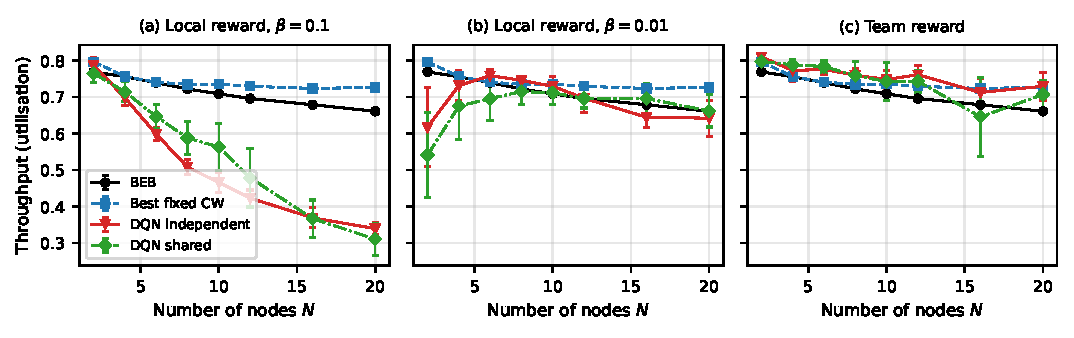
\includegraphics[width=\textwidth]{fig_throughput.pdf}
\caption{Saturation throughput versus $N$ (mean and 95\% CI over 10 seeds). The local reward collapses at high density; the team reward improves on BEB.}\label{fig:thr}
\end{figure*}
\begin{table*}[t]
\caption{Throughput, mean $\pm$ 95\% CI over 10 seeds.}\label{tab:main}
\centering\scriptsize\setlength{\tabcolsep}{3pt}
\begin{tabular}{@{}r|ccc|ccc|ccc@{}}
\toprule
 & \multicolumn{3}{c|}{Baselines} & \multicolumn{3}{c|}{Independent DQN} & \multicolumn{3}{c}{Shared-parameter DQN} \\
$N$ & BEB & Fixed & Analyt. & $\beta{=}0.1$ & $\beta{=}0.01$ & Team & $\beta{=}0.1$ & $\beta{=}0.01$ & Team \\
\midrule
2 & 0.769$\pm$0.002 & 0.796$\pm$0.002 & 0.799$\pm$0.002 & 0.786$\pm$0.022 & 0.618$\pm$0.108 & 0.809$\pm$0.006 & 0.764$\pm$0.025 & 0.541$\pm$0.117 & 0.797$\pm$0.012 \\
4 & 0.756$\pm$0.002 & 0.756$\pm$0.003 & 0.756$\pm$0.003 & 0.698$\pm$0.020 & 0.731$\pm$0.041 & 0.773$\pm$0.029 & 0.714$\pm$0.028 & 0.675$\pm$0.091 & 0.788$\pm$0.013 \\
6 & 0.739$\pm$0.002 & 0.740$\pm$0.004 & 0.745$\pm$0.003 & 0.598$\pm$0.018 & 0.758$\pm$0.018 & 0.775$\pm$0.014 & 0.646$\pm$0.033 & 0.696$\pm$0.061 & 0.783$\pm$0.017 \\
8 & 0.722$\pm$0.002 & 0.735$\pm$0.002 & 0.737$\pm$0.002 & 0.508$\pm$0.022 & 0.746$\pm$0.008 & 0.760$\pm$0.018 & 0.588$\pm$0.045 & 0.715$\pm$0.035 & 0.758$\pm$0.039 \\
10 & 0.709$\pm$0.002 & 0.735$\pm$0.002 & 0.733$\pm$0.002 & 0.466$\pm$0.027 & 0.729$\pm$0.028 & 0.748$\pm$0.025 & 0.563$\pm$0.064 & 0.712$\pm$0.032 & 0.742$\pm$0.052 \\
12 & 0.696$\pm$0.002 & 0.729$\pm$0.002 & 0.730$\pm$0.003 & 0.423$\pm$0.022 & 0.697$\pm$0.040 & 0.761$\pm$0.024 & 0.479$\pm$0.080 & 0.696$\pm$0.026 & 0.743$\pm$0.029 \\
16 & 0.679$\pm$0.003 & 0.723$\pm$0.002 & 0.727$\pm$0.002 & 0.369$\pm$0.028 & 0.644$\pm$0.027 & 0.712$\pm$0.038 & 0.367$\pm$0.051 & 0.696$\pm$0.042 & 0.646$\pm$0.107 \\
20 & 0.661$\pm$0.002 & 0.726$\pm$0.002 & 0.725$\pm$0.003 & 0.340$\pm$0.016 & 0.642$\pm$0.049 & 0.729$\pm$0.038 & 0.311$\pm$0.044 & 0.662$\pm$0.044 & 0.707$\pm$0.037 \\
\bottomrule
\end{tabular}

\end{table*}

\subsection{A. Local reward: collapse}
With $\beta{=}0.1$ both DQN variants degrade as density grows (Fig.~\ref{fig:thr}a, Table~\ref{tab:main}): at $N{=}20$ throughput is @@b01i20@@ (independent) and @@b01s20@@ (shared) against @@beb20@@ for BEB, and the collision probability reaches @@b01i20pc@@ and @@b01s20pc@@ against @@beb20pc@@. Reducing the waiting penalty to $\beta{=}0.01$ helps, but is not reliable: relative to BEB, independent DQN is significantly better only at $N\in\{@@better_b1@@\}$ and significantly worse at $N\in\{@@worse_b1@@\}$ (paired $p<0.05$), e.g.\ @@b001i2@@ against @@beb2@@ at $N{=}2$. At $N{=}20$ the mean chosen CW is only @@cw20_i001@@ whereas the analytic optimum is @@cw20_a@@. Shared parameters do not remove the problem.

\subsection{B. Team reward: improvement, with caveats}
With the team reward (Fig.~\ref{fig:thr}c) independent DQN improves the mean throughput over BEB at every tested $N$, by @@dmin@@ to @@dmax@@; the improvement is significant ($p<0.01$) at $N\in\{@@sig_i@@\}$ (Table~\ref{tab:team}). At $N{=}20$ it reaches @@ti20@@ versus @@beb20@@ for BEB and @@fix20@@ for the best fixed CW. It is statistically indistinguishable from the best fixed CW at $N\in\{@@tie_i@@\}$ and significantly above it at $N\in\{@@above_fix_i@@\}$ ($p<0.05$). Shared-parameter DQN improves on BEB significantly at $N\in\{@@sig_s@@\}$ (@@ts20@@ at $N{=}20$, $\Delta S{=}@@ds20@@$, $p{=}@@ps20@@$) but is less stable across seeds at high density and does not reach the best fixed CW there.

\begin{table}[t]
\caption{Team reward: paired throughput difference to BEB ($\Delta S$, paired $t$-test $p$) and Jain fairness index.}\label{tab:team}
\centering\scriptsize\setlength{\tabcolsep}{3pt}
\begin{tabular}{@{}rcccccc@{}}
\toprule
 & \multicolumn{3}{c}{Independent DQN} & \multicolumn{3}{c}{Shared-parameter DQN} \\
$N$ & $\Delta S$ vs BEB & $p$ & Jain & $\Delta S$ vs BEB & $p$ & Jain \\
\midrule
2 & +0.041 & $<$0.001 & 0.91 & +0.028 & $<$0.001 & 0.99 \\
4 & +0.017 & 0.217 & 0.70 & +0.033 & $<$0.001 & 0.98 \\
6 & +0.036 & $<$0.001 & 0.60 & +0.044 & $<$0.001 & 0.96 \\
8 & +0.038 & 0.001 & 0.43 & +0.036 & 0.069 & 0.94 \\
10 & +0.039 & 0.006 & 0.34 & +0.034 & 0.185 & 0.96 \\
12 & +0.065 & $<$0.001 & 0.27 & +0.047 & 0.006 & 0.95 \\
16 & +0.034 & 0.083 & 0.27 & -0.033 & 0.504 & 0.95 \\
20 & +0.069 & 0.003 & 0.19 & +0.046 & 0.020 & 0.94 \\
\bottomrule
\end{tabular}

\end{table}
\begin{figure*}[t]
\centering
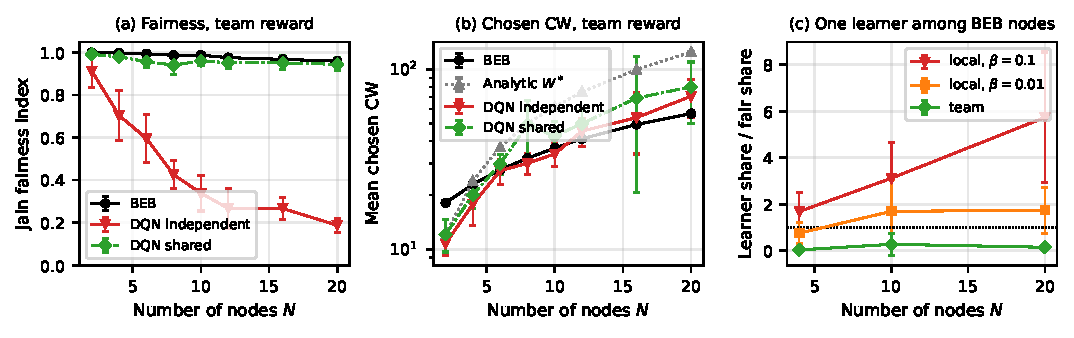
\includegraphics[width=\textwidth]{fig_fair.pdf}
\caption{(a) Fairness and (b) mean chosen CW under the team reward. (c) Share of successes won by a single learner among $N{-}1$ BEB nodes, relative to the fair share $1/N$ (dotted line).}\label{fig:fair}
\end{figure*}

\subsection{C. The throughput of independent agents comes at a fairness cost}
Under the team reward independent agents are very unequal: the Jain index falls from @@jti10@@ at $N{=}10$ to @@jti20@@ at $N{=}20$ (Fig.~\ref{fig:fair}a), whereas BEB and the static references stay above 0.95. Unequal allocation can raise total throughput, because a few nodes capture the channel while others back off, so the throughput of independent agents should not be read without the fairness index. Shared parameters give every node the same policy and preserve fairness (@@jts10@@ at $N{=}10$, @@jts20@@ at $N{=}20$). The mean chosen CW at $N{=}20$ is @@cw20_i@@ (independent) and @@cw20_s@@ (shared), between BEB (@@cw20_b@@) and the analytic optimum (@@cw20_a@@) (Fig.~\ref{fig:fair}b).

\subsection{D. One learner among BEB nodes}
To see what a single reward does to behaviour, one node runs a DQN and the other $N{-}1$ run BEB. System throughput stays close to that of BEB (within @@one_dev@@ for $N\ge 10$ in all three reward settings), but the learner's share of successes does not (Fig.~\ref{fig:fair}c). Under the local reward with $\beta{=}0.1$ it wins @@sh10_01@@ and @@sh20_01@@ times its fair share at $N{=}10, 20$, which is greedy behaviour. With $\beta{=}0.01$ it wins about @@sh20_001@@ times its fair share at $N{=}20$, and with the team reward only @@sh10_t@@ and @@sh20_t@@ times, which is altruistic behaviour. Hence the local reward teaches an agent to benefit itself at the expense of others, and when all agents do so the channel collapses (Section~V-A).

\section{Discussion and Limitations}
\textbf{Mechanism.} The collapse under the local reward is consistent with a misaligned incentive: waiting is penalised, collisions are penalised only once, and an agent does not pay for the collisions it causes to others. The one-learner experiment supports this reading, but we did not vary the reward further, so we regard the waiting penalty as the likely rather than the proven cause. We also did not separate non-stationarity from reward misalignment with a dedicated experiment; the fact that parameter sharing alone does not help under the local reward, while changing the reward does, points to the reward as the dominant factor in this setting.

\textbf{Limitations.} (i) Traffic is saturated, the network is a single collision domain, and the PHY is ideal; hidden terminals, unsaturated traffic and IEEE 802.15.4 are not studied. (ii) The values $\beta\in\{0.1,0.01\}$ and the team-reward scale were selected after short pilot runs ($N{=}10$, two seeds) that reused training seeds~0 and~1; the evaluation environments differ, but the choice is not a clean held-out selection. (iii) The team reward requires global information during training, which a deployment must provide. (iv) We compare against BEB and static references, not against other learned MAC protocols or CTDE algorithms such as QMIX. (v) The fairness of independent agents is poor and a fairness-aware reward was not evaluated. (vi) Shared-parameter training is unstable at $N\ge 16$; longer training and more seeds are needed there.

\section{Conclusion}
In a validated slotted CSMA/CA simulator, DQN contention-window agents either collapse or improve on BEB depending mainly on their reward. A local, waiting-time-weighted reward makes agents greedy and the channel collapse at high density, whereas a team reward lets independent agents beat BEB and match the best static CW, at a large fairness cost that parameter sharing largely removes. Future work should evaluate fairness-aware rewards, unsaturated traffic, CTDE algorithms, and IEEE 802.15.4. The simulator and experiment scripts are available at \url{https://github.com/hesamAmiri04/ai-csma-simulator}.

\begin{thebibliography}{10}
\bibitem{bianchi2000} G.~Bianchi, ``Performance analysis of the IEEE 802.11 distributed coordination function,'' \emph{IEEE J. Sel. Areas Commun.}, vol.~18, no.~3, pp. 535--547, 2000.
\bibitem{amuru2015} S.~Amuru, Y.~Xiao, M.~van der Schaar, and R.~M. Buehrer, ``To send or not to send -- learning MAC contention,'' in \emph{Proc. IEEE GLOBECOM}, 2015, pp. 1--6.
\bibitem{wydmanski2021} W.~Wydma\'nski and S.~Szott, ``Contention window optimization in IEEE 802.11ax networks with deep reinforcement learning,'' in \emph{Proc. IEEE WCNC}, 2021.
\bibitem{yu2019} Y.~Yu, T.~Wang, and S.~C. Liew, ``Deep-reinforcement learning multiple access for heterogeneous wireless networks,'' \emph{IEEE J. Sel. Areas Commun.}, vol.~37, no.~6, pp. 1277--1290, 2019.
\bibitem{mnih2015} V.~Mnih \emph{et al.}, ``Human-level control through deep reinforcement learning,'' \emph{Nature}, vol. 518, pp. 529--533, 2015.
\bibitem{hernandez2017} P.~Hernandez-Leal, M.~Kaisers, T.~Baarslag, and E.~M. de~Cote, ``A survey of learning in multiagent environments: Dealing with non-stationarity,'' arXiv:1707.09183, 2017.
\bibitem{tampuu2017} A.~Tampuu \emph{et al.}, ``Multiagent cooperation and competition with deep reinforcement learning,'' \emph{PLoS ONE}, vol.~12, no.~4, e0172395, 2017.
\bibitem{lowe2017} R.~Lowe \emph{et al.}, ``Multi-agent actor-critic for mixed cooperative-competitive environments,'' in \emph{Proc. NeurIPS}, 2017.
\bibitem{rashid2018} T.~Rashid \emph{et al.}, ``QMIX: Monotonic value function factorisation for deep multi-agent reinforcement learning,'' in \emph{Proc. ICML}, 2018.
\bibitem{jain1984} R.~Jain, D.-M. Chiu, and W.~R. Hawe, ``A quantitative measure of fairness and discrimination for resource allocation in shared computer systems,'' DEC Research Report TR-301, 1984.
\end{thebibliography}
\end{document}
